\documentclass{beamer}
\usepackage{graphicx}
\usepackage{graphics}
\usepackage{hyperref}
\usepackage[english]{babel}
\usepackage[T1]{polski}
\usepackage{multimedia}

\renewcommand{\figurename}{Fig.}
\addto\captionsenglish{\renewcommand{\figurename}{}}
\usepackage[font=scriptsize]{caption}

\mode<presentation>
{
    \usetheme{AMUFree-kk}
    \setbeamercovered{transparent = 28}
}
\title{History of the forbidden model}
\author[{K. Kaczmarek}]{Karol Kaczmarek}
\date{2019}
\setbeamertemplate{bibliography item}{[\theenumiv]}

\begin{document}

\begin{frame}
    \titlepage
\end{frame}

\AtBeginSection[]
{
    \begin{frame}
        \frametitle{Outline}
        \tableofcontents[currentsection]
    \end{frame}
}


\section{Transformer}

\begin{frame}
    \frametitle{Transformer - Architecture}
    \begin{itemize}
        \item publication: "Attention Is All You Need" \cite{transformer}
        \item encoder-decoder model
        \item dispensing with recurrence and convolutions entirely
        \item attention mechanism
    \end{itemize}
\end{frame}

\begin{frame}
    \frametitle{Transformer - Architecture}
    \begin{center}
        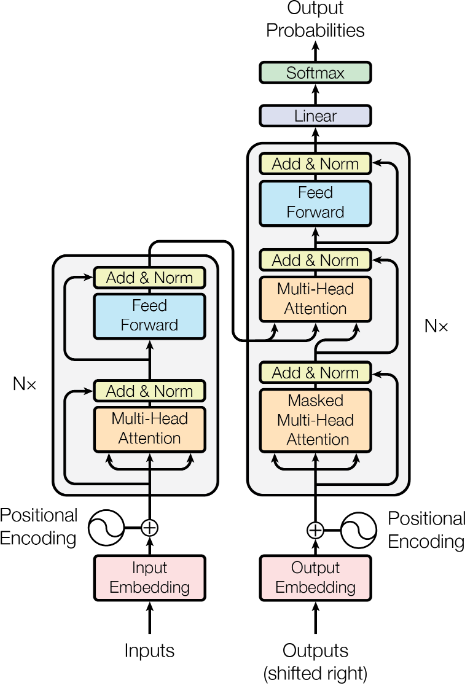
\includegraphics[scale=1.15]{img/transformer.png}
    \end{center}
\end{frame}

\begin{frame}
    \frametitle{Transformer - Architecture}
    \begin{center}
        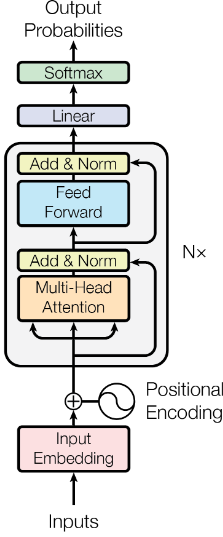
\includegraphics[scale=1.4]{img/transformer_lm.png}
    \end{center}
\end{frame}

\begin{frame}
    \frametitle{Transformer - Positional Encoding}
    \begin{itemize}
    	\item position of the word in the text (at the beginning or at the end)
    	\item add \textit{positional encodings} to the \textit{input embeddings}
        \item $ PE_{(pos, 2i)} = sin(pos / 10000^{2i/d_{model}} ) $
        \item $ PE_{(pos, 2i+1)} = cos(pos / 10000^{2i/d_{model}} ) $
        \begin{itemize}
        	\item $ pos $ - position
        	\item $ i $ - dimension 
        	\item $ d_{model} $ - dimension embeddings
        \end{itemize}
    \end{itemize}
\end{frame}

\begin{frame}
    \frametitle{Transformer - Positional Encoding}
    \begin{center}
        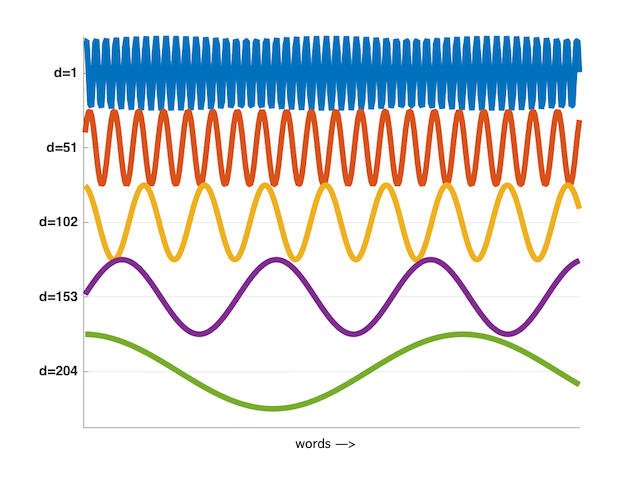
\includegraphics[scale=0.425]{img/positional_encodings.png}
    \end{center}
\end{frame}

\begin{frame}
    \frametitle{Transformer - Attention}
    \begin{itemize}
        \item attention function can be described as mapping a \textit{query} and a set of \textit{key-value} pairs to an \textit{output}, where:
        \begin{itemize}
        	\item $ Q $ - queries matrix
        	\item $ K $ - keys matrix
        	\item $ V $ - values matrix
        \end{itemize}
    \end{itemize}
\end{frame}

\begin{frame}
    \frametitle{Transformer - Multi-head attention}
    \begin{center}
        \item $ Attention (Q, K, V) = softmax(\frac{QK^T}{\sqrt{d_k}})V $
        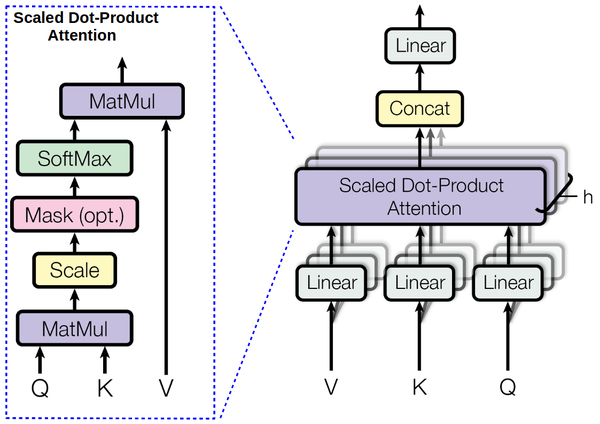
\includegraphics[scale=0.45]{img/multi_head_attention.png}
    \end{center}
\end{frame}

\begin{frame}
    \begin{center}
        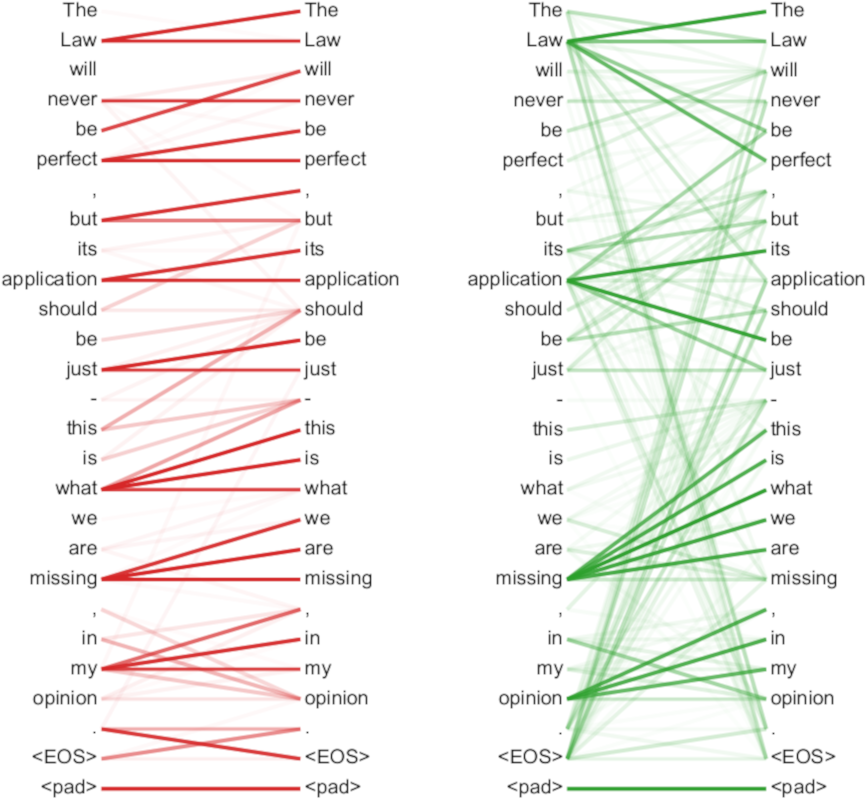
\includegraphics[scale=1.2]{img/transformer_att_sentence.png}
    \end{center}
\end{frame}

\begin{frame}
    \frametitle{Transformer - Visualization}
	\movie[autostart,showcontrols,height=0.5\textwidth ,width=\textwidth]{}{img/transform20fps.mp4}
\end{frame}

\begin{frame}
    \frametitle{Transformer - Visualization}
	\movie[autostart,showcontrols,height=0.5\textwidth ,width=\textwidth]{}{img/transformer_att.mp4}
\end{frame}



\section{GLUE Benchmark}

\begin{frame}
    \frametitle{GLUE Benchmark \cite{glue}}
    \begin{itemize}
        \item \textbf{GLUE} -- \textbf{G}eneral \textbf{L}anguage \textbf{U}nderstanding \textbf{E}valuation
        \item \textbf{N}atural \textbf{L}anguage \textbf{U}nderstanding tasks (NLU):
        \begin{itemize}
			\item single-sentence tasks: CoLA, SST-2
			\item similarity and paraphrase tasks: MRPC, STS-B, QQP
			\item inference tasks: MNLI, QNLI, RTE, WNLI
        \end{itemize}
    \end{itemize}
\end{frame}

\begin{frame}
    \frametitle{GLUE Benchmark - Leaderboard}
    \begin{center}
    	\begin{tabular}{l | c}
    		\textbf{Name} & \textbf{Score} \\
    		\hline
    		Human & $ 87.1 $ \\
    		ALICE large (Alibaba DAMO NLP) & $ 82.9 $ \\
    		MT-DNNv2 (Microsoft D365 AI) & $ 82.9 $ \\
    		BERT & $ 82.0-80.2 $ \\
    		Transformer & $ 72.8 $ \\
    		ELMO & $ 70.5 $ \\
    		Baseline & $ \sim 70.0 $
    	\end{tabular}
    \end{center}
\end{frame}

\begin{frame}
    \frametitle{GLUE Benchmark - Leaderboard}
    \begin{center}
        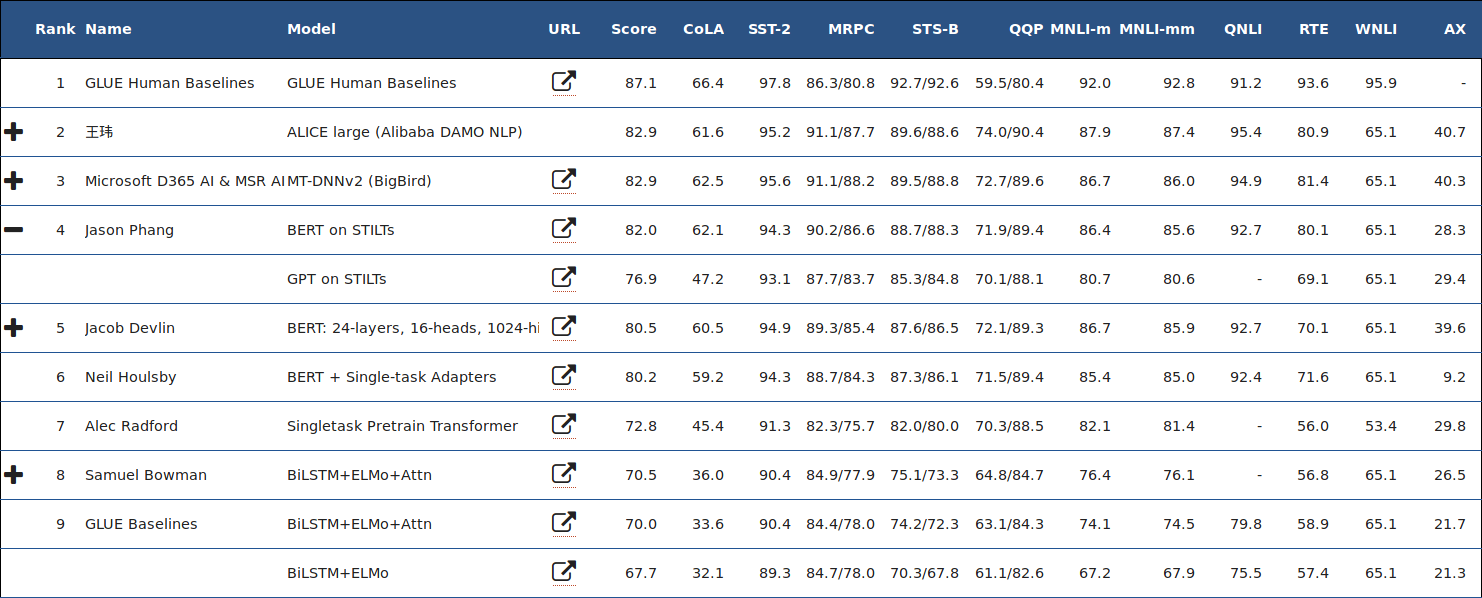
\includegraphics[scale=0.9]{img/glue_leaderboard.png}
    \end{center}
\end{frame}

\begin{frame}<presentation:0>
    \frametitle{Score DEV}
    \begin{center}
        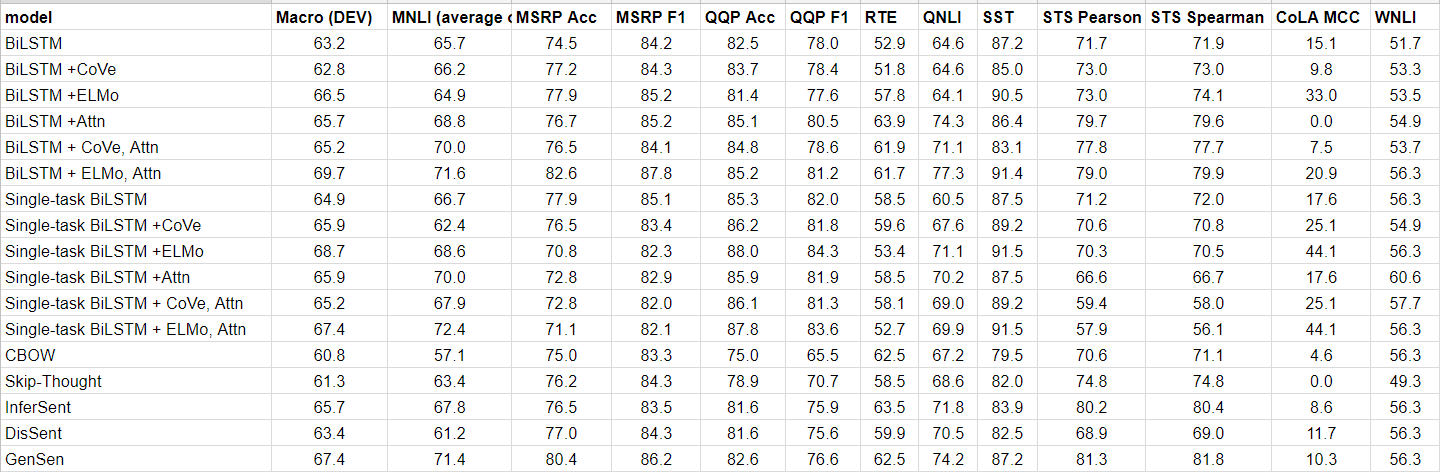
\includegraphics[scale=0.22]{img/glue_dev.png}
        
\includegraphics[scale=1.132]{img/glue_my.png}
    	% {'CoLA': 16.81, 'RTE': 58.48, 'QQP': {'f1': 66.29, 'acc': 74.34}, 'QNLI': 67.17, 'MNLI': 53.12, 'WNLI': 56.34, 'STSBenchmark': {'sr': 63.97, 'pr': 63.28}, 'SST2': 78.33, 'MRPC': {'f1': 82.33, 'acc': 74.75}, 'MACRO': 60.3}
    \end{center}
\end{frame}


% https://lilianweng.github.io/lil-log/2019/01/31/generalized-language-models.html
\section{BERT}

\begin{frame}
    \frametitle{BERT \cite{bert}}
    \begin{itemize}
        \item \textbf{BERT} -- \textbf{B}idirectional \textbf{E}ncoder \textbf{R}epresentations from \textbf{T}ransformers = bidirectional Transformers
    \end{itemize}
    \begin{center}
        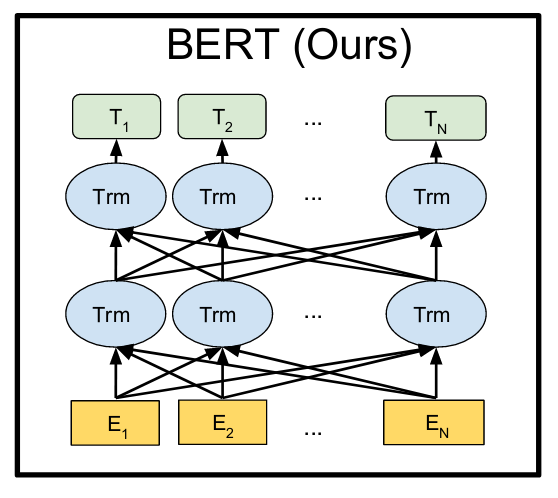
\includegraphics[scale=1.0]{img/bert.png}
    \end{center}
\end{frame}

\begin{frame}
    \frametitle{BERT - Input representation}
    \begin{itemize}
        \item \textbf{[CLS]} -- the special classification embedding
        \item \textbf{[SEP]} -- sentences separator, sentence pairs are packed together into a single sequence
        \item segment embeddings
    \end{itemize}
    \begin{center}
        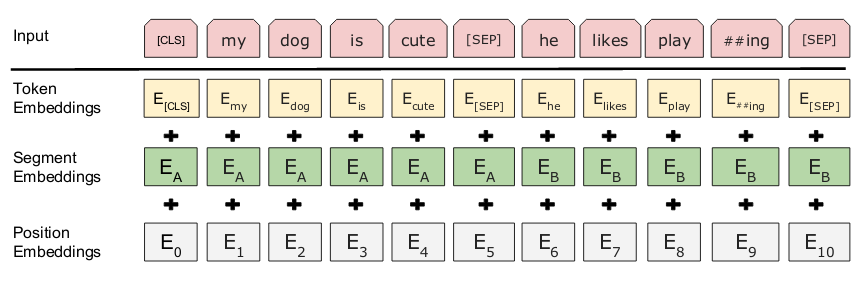
\includegraphics[scale=1.4]{img/bert_input.png}
    \end{center}
\end{frame}

\begin{frame}
    \frametitle{Masked Language Model (MLM)}
    \begin{itemize}
        \item masking some percentage of the input tokens at random
        \item predicting only those masked tokens (\textbf{[MASK]})
        \item mask 15\% of all
        \item masking procedure:
        \begin{itemize}
        	\item 80\% of the time - replace the word with the \textbf{[MASK]} token
        	\begin{itemize}
        		\item \textit{my dog is hairy $\rightarrow$ my dog is [MASK]}
        	\end{itemize}
        	\item 10\% of the time - replace the word with a random word
        	\begin{itemize}
        		\item \textit{my dog is hairy $\rightarrow$ my dog is apple}
        	\end{itemize}
        	\item 10\% of the time - keep the word  unchanged
        	\begin{itemize}
        		\item \textit{my dog is hairy $\rightarrow$ my dog is hairy}
        	\end{itemize}
        \end{itemize}
    \end{itemize}
\end{frame}


\section{Forbidden model}

\begin{frame}
    \begin{figure}
        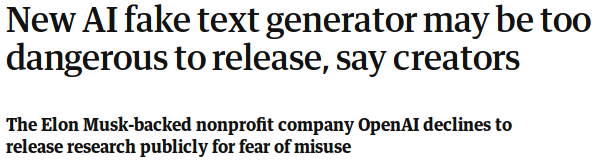
\includegraphics[scale=0.8]{img/gpt2_en1.png}
    	\caption{theguardian.com}
    \end{figure}
    \begin{figure}
       	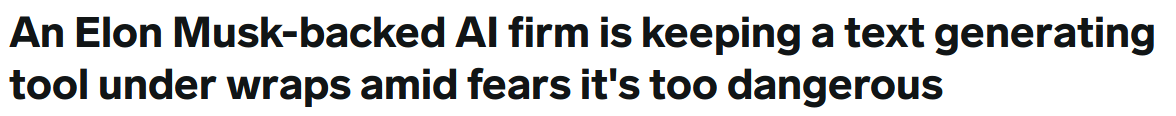
\includegraphics[scale=0.8]{img/gpt2_en2.png}
    	\caption{businessinsider.com}
    \end{figure}
    \begin{figure}
       	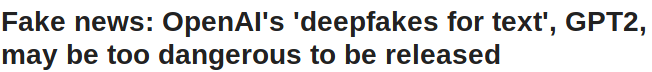
\includegraphics[scale=0.8]{img/gpt2_en3.png}
    	\caption{betanews.com}
    \end{figure}
    \begin{figure}
       	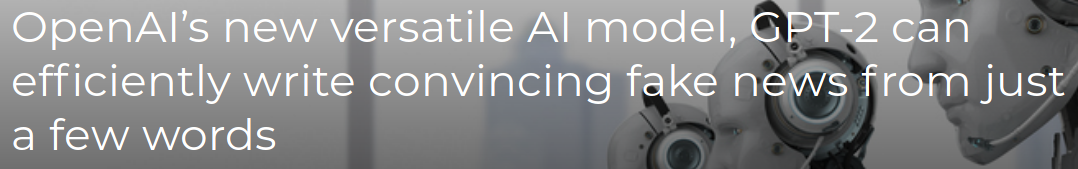
\includegraphics[scale=0.8]{img/gpt2_en4.png}
    	\caption{packtpub.com}
    \end{figure}
\end{frame}

\begin{frame}
    \begin{figure}
        
\includegraphics[scale=0.8]{img/gpt2_pl1.png}
    	\caption{rp.pl}
    \end{figure}
    \begin{figure}
       	
\includegraphics[scale=0.8]{img/gpt2_pl2.png}
    	\caption{polityka.pl}
    \end{figure}
    \begin{figure}
       	
\includegraphics[scale=0.8]{img/gpt2_pl3.png}
    	\caption{ithardware.pl}
    \end{figure}
    \begin{figure}
       	
\includegraphics[scale=0.8]{img/gpt2_pl4.png}
    	\caption{giznet.pl}
    \end{figure}
\end{frame}

\begin{frame}
    \begin{center}
        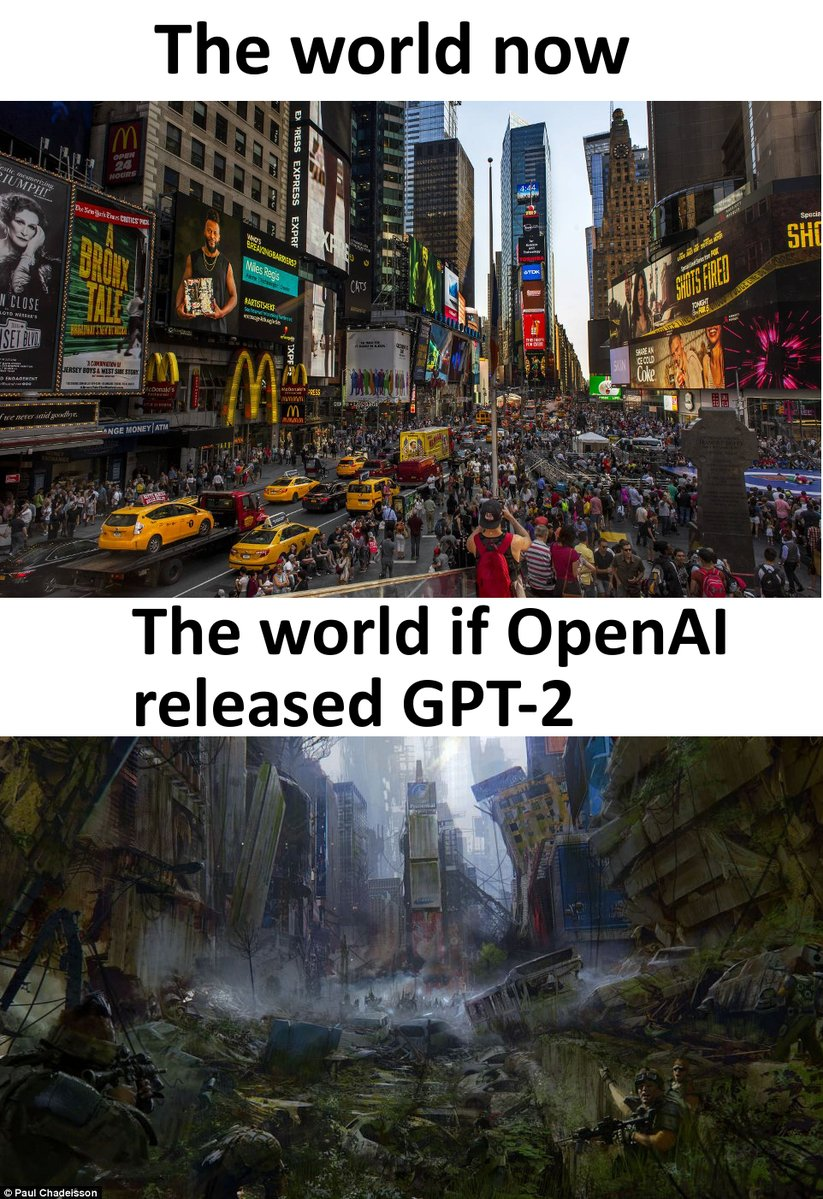
\includegraphics[scale=0.18]{img/gpt2_mem1.jpg}
    \end{center}
\end{frame}


% https://openai.com/blog/better-language-models/
\section{GPT-2}

\begin{frame}
    \frametitle{GPT-2 \cite{gpt2}}
    \begin{itemize}
        \item transformer-based language model
        \item training dataset (WebText):
        \begin{itemize}
			\item scrapted web pages which have been curated/filtered by humans
        	\item links from \textit{reddit}, which received at least 3 karma
        	\item 45 million links = 8 million documents = 40 GB of text
        	\item removed all Wikipedia documents
        \end{itemize}
        \item using Byte Pair Encoding (BPE)
        \item 1 of 4 models have been published (117M, 345M, 762M, 1542M)
        \item training the big GPT-2 model costs \$43k
        \item OpenWebText
    \end{itemize}
\end{frame}

\begin{frame}
    \frametitle{Byte Pair Encoding (BPE)}
    \begin{itemize}
        \item often operate of Unicode code points (vocabulary of over 130000, usually 32000-64000)
        \item operate of byte-level only required a base vocabulary of size 256
        \item generating multiple versions of common words (\textit{dog.} \textit{dog!} \textit{dog?} for the word \textit{dog})
        \item prevents BPE from merging characters across categories (\textit{dog} would not be merged with punctuation characters)
        \item $<$UNK$>$ occurring only 26 times in 40 billion bytes
        \item do not need to worry about pre-processing, tokenization
	\end{itemize}
\end{frame}

\begin{frame}
    \frametitle{GPT-2 - Model size}
    \begin{center}
        \begin{tabular}{ l | c | c | c }
        \textbf{Name} & \textbf{Parameters} & \textbf{Layers} & \textbf{Dimensions}\\
        & & ($L$) & ($d_{model}$)\\
        \hline
        \textbf{base} & 117M & 12 & 768\\
        \textbf{medium} & 345M & 24 & 1024\\
        \textbf{large} & 762M & 36 & 1280\\
        \textbf{xl} & 1542M & 48 & 1600\\
        \end{tabular}
    \end{center}
\end{frame}

\begin{frame}
    \frametitle{GPT-2 - Score}
    \begin{center}
        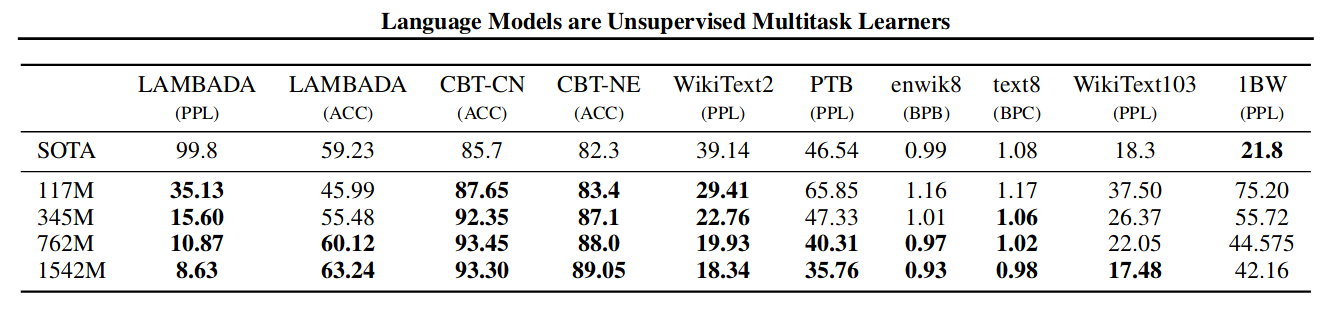
\includegraphics[scale=1.0]{img/gpt2_score.png}
    \end{center}
\end{frame}

\begin{frame}
	\begin{itemize}
		\item[] \textbf{Human written}: In a shocking finding, scientist discovered a herd of unicorns living in a remote, previously unexplored valley, in the Andes Mountains. Even more surprising to the researchers was the fact that the unicorns spoke perfect English.
		\item[] \textbf{Model completion}: The scientist named the population, after their distinctive horn, Ovid’s Unicorn. These four-horned, silver-white unicorns were previously unknown to science.
		\item[] Now, after almost two centuries, the mystery of what sparked this odd phenomenon is finally solved.
		\item[] Dr. Jorge Pérez, an evolutionary biologist from the University of La Paz, and several companions, were exploring the Andes Mountains when they found a small valley, with no other animals or humans. Pérez noticed that the valley had what appeared to be a natural fountain, surrounded by two peaks of rock and silver snow.
	\end{itemize}
\end{frame}

\begin{frame}
    \begin{center}
    \begin{figure}
        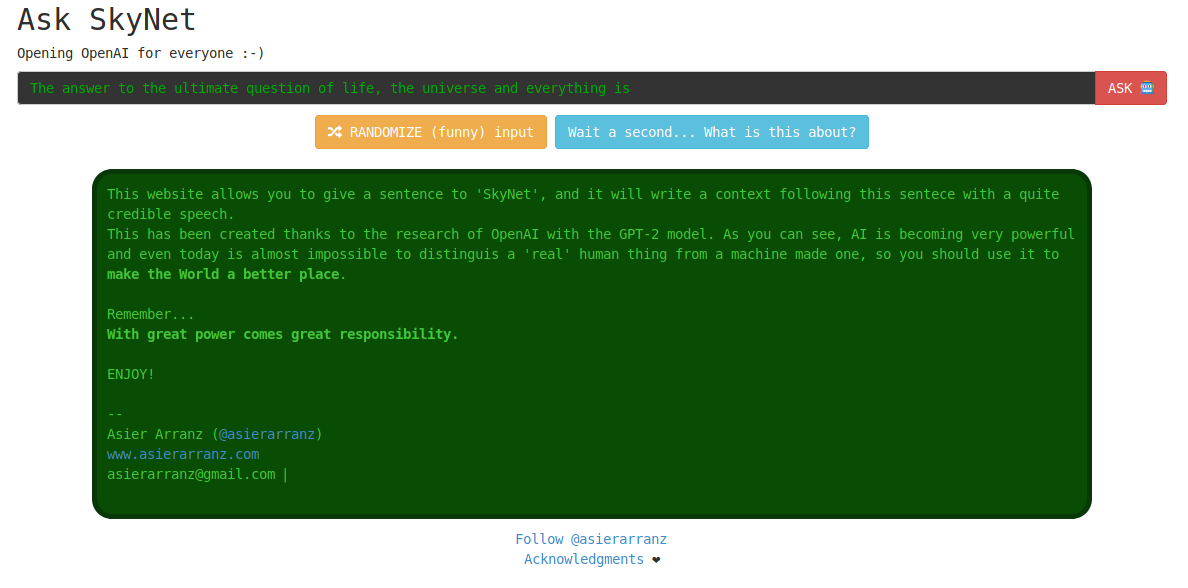
\includegraphics[scale=1.1]{img/ask_skynet.png}
    	\caption{askskynet.com}
    \end{figure}
    \end{center}
\end{frame}


\section{Examples}

\begin{frame}
    \frametitle{Transformer on Polish CommonCrawl}
	\begin{itemize}
		\item[] Jarosław Kaczyński , przewodniczący PiS i kandydat Prawa ręka - mówił szef Biura Rady Miejskiej Robert Miller zapowiedział , że szef PiS złożył na niego list , by minister sprawiedliwości Jacek Giertych o jego kadencji minister właściwy z dniem 11 l i
	\end{itemize}
\end{frame}


% References
\section{References}
\begin{frame}[allowframebreaks,t]
    \tiny
    \frametitle{References}
    \bibliographystyle{ieeetr}
    \bibliography{gpt_2}
    %\nocite{*}
\end{frame}

\end{document}
